\documentclass[onecolumn]{article}
\usepackage{graphicx}
\usepackage{float}
\restylefloat{figure}
\begin{document}

\title{Do bounded functions always have a "statistical" average?}

\author{Arjen Markus}

\maketitle

\section*{Introduction}
When applying statistical techniques, we usually take a lot for granted:
the time series is often assumed stationary and otherwise we look for reasons
why it is not. Data are independent and so on. We also assume that a time series
has an average. Since the time series is almost always finite (and the
individual data as well), this is trivial. But what about mathematical
functions? Of course, functions that tend to infinity cannot have a finite
average, but intuitively, one would assume that for bounded functions
averages always exist. In this note I want to explore this assumption.

\section*{A counter example}
Consider the function:
\begin{eqnarray}
             f(x) &=& 1 ~~~~\textrm{if} ~2^{2n} < x \leq 2^{2n+1}   \\
\nonumber         &=& 0 ~~~~\textrm{if} ~2^{2n+1} < x \leq 2^{2n+2} \\
\nonumber         &=& 0 ~~~~\textrm{if} ~x \leq 1
\end{eqnarray}
\noindent where $n$ is a positive integer.

The function is illustrated below:
\begin{figure}[H]
\caption{Function with exponentially sized intervals}
\label{expfunc}
\begin{center}
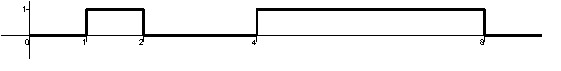
\includegraphics[width=0.9\textwidth]{bounded.pdf}
\end{center}
\end{figure}

The average of the function over the intervl $[0,T]$ is:
\begin{equation}
    F(T) = \frac{1}{T} \int\limits_{0}^{T} f(x) dx
\end{equation}

The easiest way to evaluate this integral and determine the limit for
$T \rightarrow \infty$ is to determine the contribution of each interval.

For $T = 2^{2n+1}$:
\begin{eqnarray}
    F(T) = F(2^{2n+1}) &=& \frac{1}{2^{2n+1}} \bigl ( 2^{2n}F(2^{2n}) + (2^{2n+1} - 2^n) \bigr ) \\
\nonumber              &=& \frac{1}{2} (F(2^{2n}) + \frac{1}{2}
\end{eqnarray}

For $T = 2^{2n+2}$:
\begin{eqnarray}
    F(T) = F(2^{2n+2}) &=& \frac{1}{2^{2n+2}} \bigl ( 2^{2n+1}F(2^{2n+1}) \bigr ) \\
\nonumber              &=& \frac{1}{2} F(2^{2n+1})
\end{eqnarray}

Straightfoward manipulation of these relations gives:
\begin{eqnarray}
\label{recodd}
    F(2^{2n+1}) &=& \frac{1}{4} F(2^{2n-1}) + \frac{1}{2} \\
\label{receven}
    F(2^{2n+2}) &=& \frac{1}{4} F(2^{2n}) + \frac{1}{4}
\end{eqnarray}

For notational convenience we use the following auxiliary functions, $O(n)$ (odd) and $E(n)$ (even):
\begin{eqnarray}
    O(n) &=& F(2^{2n+1}) \\
    E(n) &=& F(2^{2n})
\end{eqnarray}
Then the recurrence relations \ref{recodd} and \ref{receven} become:
\begin{eqnarray}
    O(n) &=& \frac{1}{4} O(n-1) + \frac{1}{2} \\
    E(n) &=& \frac{1}{4} E(n-1) + \frac{1}{4}
\end{eqnarray}

The initial conditions for $n = 0$, as can be read from Figure \ref{expfunc} are: $E(0) = 0$ and $O(0) = \frac{1}{2}$, as the
function $f$ is 0 in the interval [0,1) ($= 2^0$) and is 1 in the interval [1,2). This makes the solution of the
above recursive relations easy to find. The general form is:
\begin{eqnarray}
    O(n) &=& A \lambda^{n} + B
\end{eqnarray}
With the initial conditions we find:
\begin{eqnarray}
    O(n) &=& -\frac{1}{6} \bigl (\frac{1}{4} \bigr )^n + \frac{2}{3} \\
    E(n) &=& -\frac{1}{3} \bigl ( \frac{1}{4} \bigr )^n + \frac{1}{3}
\end{eqnarray}
Hence the integral, sampled at these different points, converges to two different values: $\frac{1}{3}$ and $\frac{2}{3}$.

Thus the above function does not have a particular average in the limit.

\section*{Another counter example?}
The fact that the intervals over which the function from the previous section grow exponentially leads to the question
whether it is necessary that they grow so fast or whether a slower growth, for example as some power, is sufficient.

So, consider the function, as illustrated in Figure \ref{quadfunc}:
\begin{eqnarray}
             f(x) &=& 1 ~~~~\textrm{if} ~(2n)^2 < x \leq (2n+1)^2   \\
\nonumber         &=& 0 ~~~~\textrm{if} ~(2n+1)^2 < x \leq (2n+2)^2 \\
\nonumber         &=& 0 ~~~~\textrm{if} ~x \leq 1
\end{eqnarray}
\noindent where $n$ is a positive integer.

\begin{figure}[H]
\caption{Function with quadratically sized intervals}
\label{quadfunc}
\begin{center}
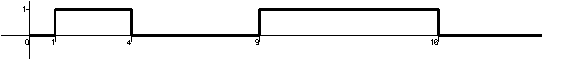
\includegraphics[width=0.9\textwidth]{bounded_2.pdf}
\end{center}
\end{figure}

For the values of $x = (2n)^2$ the integral can be written as:
\begin{eqnarray}
    F\bigl( (2n)^2 \bigr) &=& \frac{1}{(2n)^2} \sum_{k=1}^n \bigl( (2k)^2 - (2k-1)^2 \bigr) \\
\nonumber                 &=& \frac{1}{(2n)^2} \sum_{k=1}^n (4k - 1) \\
\nonumber                 &=& \frac{1}{(2n)^2} \bigl( 2n^2 - n \bigr) = \frac{2n - 1}{4n}
\end{eqnarray}

Similarly, for the values of $x = (2n+1)^2$ the integral can be written as:
\begin{eqnarray}
    F\bigl( (2n+1)^2 \bigr) &=& \frac{1}{(2n+1)^2} \sum_{k=1}^n \bigl( (2k)^2 - (2k-1)^2 \bigr) \\
\nonumber                   &=& \frac{1}{(2n+1)^2} \bigl( 2n^2 - n \bigr) = \frac{2n^2 - n}{(2n+1)^2}
\end{eqnarray}

For this second function the average integral converges slowly to $\frac{1}{2}$ in both cases.
On the basis of the above analysis we can also conclude that intervals that grow as polynomials
will not induce the splitted limits of the exponentially growing intervals from the first section.
Substantially faster growth is required.

\end{document}

